\section{异步通信中断接收实现}
一台机子使用中断发送,一台机子使用中断接收。
\subsection{原理分析}
在异步通信中断发送实现的基础上,打开uart0的中断,以用于中断接收,并用led来展示。\\
\\
原理图如下:\\
\begin{figure}[htbp]
  \centering
  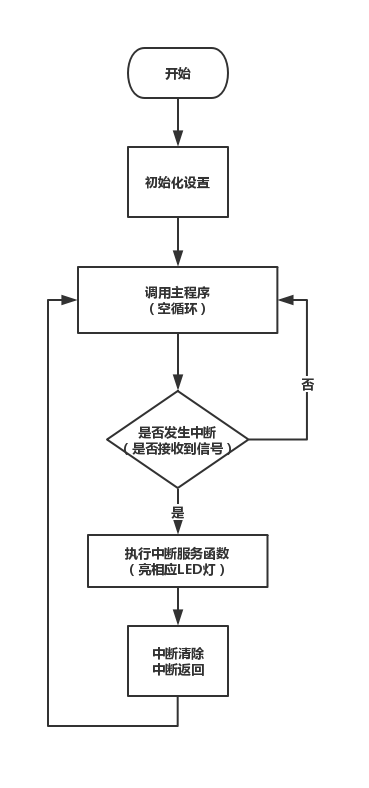
\includegraphics[width=0.3\textwidth]{sch5.png}
  \caption{异步通信中断接收实现原理图}
\end{figure}
\\

\subsection{调试过程}
\subsubsection{UART寄存器分析}
打开\lstinline{s3c24xx.h},这里使用到的interrupt registes,我们可以看到
\lstset{language=C}

\begin{lstlisting}{UART寄存器分析}
    /*UART registers*/
    #define ULCON0              (*(volatile unsigned long *)0x50000000)
    #define UCON0               (*(volatile unsigned long *)0x50000004)
    #define UFCON0              (*(volatile unsigned long *)0x50000008)
    #define UMCON0              (*(volatile unsigned long *)0x5000000c)
    #define UTRSTAT0            (*(volatile unsigned long *)0x50000010)
    #define UTXH0               (*(volatile unsigned char *)0x50000020)
    #define URXH0               (*(volatile unsigned char *)0x50000024)
    #define UBRDIV0             (*(volatile unsigned long *)0x50000028)
    
\end{lstlisting}
这里使用了大量UART相关寄存器,后面会详细分析。

\subsubsection{UART寄存器配置}
打开\lstinline{init.c},这里对中断寄存器配置,我们可以看到
\lstset{language=C}
\begin{lstlisting}{中断寄存器配置}
    void init_irq( )
    {
        SUBSRCPND |= 0x3;
        SRCPND |= 0x1<<28;
        INTPND |= 0x1<<28;
    
        INTSUBMSK &= ~(0x1);
        INTSUBMSK |= (0x1<<1);
        INTMSK &= ~(0x1<<28);
    }
\end{lstlisting}

\lstset{language=C}
\begin{lstlisting}{中断寄存器配置}
    void uart0_init(void)
    {
        GPHCON&=0x3c0000;
        GPHCON|=0x2faaa;
        GPBCON = 0x1dd7fc;//GPB5,6,8,10设置为输出
        GPBDAT|=0x560;//4个LED全灭
        GPHUP=0x1ff;//H口上拉禁止
        GPFCON &=~((3<<0)|(3<<4)|(3<<6)|(3<<8)) ;
        GPFCON |= ((2<<0)|(2<<4)|(2<<6)|(2<<8)) ;//GPF0,GPF2,GPF3,GPF4工作在第二功能状态,即中断
        EINTPEND=(1<<4);
    
        
        ULCON0 &=0XFFFFFF00;
        ULCON0 |=0X03;      // 8N1(8个数据位,无较验,1个停止位)
        UCON0   = 0x09;     // 中断请求
        UFCON0  = 0x00;     // 不使用FIFO
        UMCON0  = 0x00;     // 不使用流控
        UBRDIV0 = UART_BRD; // 波特率为115200
    }

\end{lstlisting}
配置分析:
UART 线路控制寄存器: \\
我们选取8个数据位,无较验,1个停止位\\
 \begin{figure}[h]
    \centering
    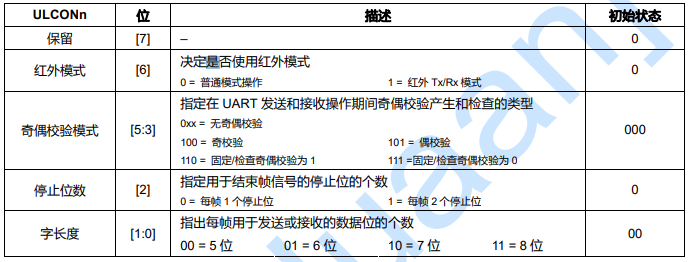
\includegraphics[width=0.7\textwidth]{uart2.png}
    \caption{ULCON0}
\end{figure}
UART 控制寄存器: \\
选取1 = 电平(当非 FIFO 模式中 Tx 缓冲器为空或 FIFO 模式中达到 Tx FIFO 触发深度时请
求中断),并且UFCON0寄存器中,不使用FIFO。UMCON0中,不使用流控。\\
\begin{figure}[h]
    \centering
    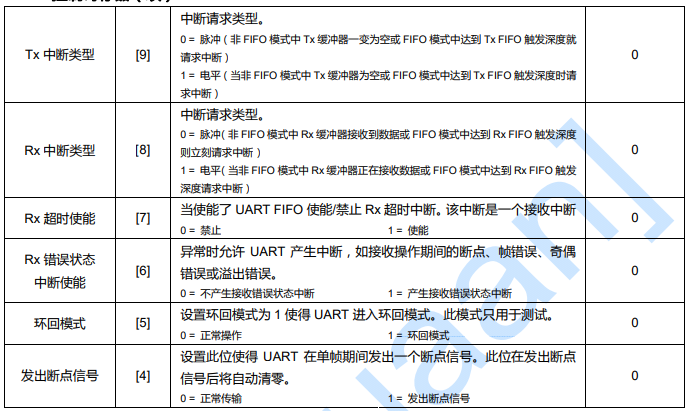
\includegraphics[width=0.7\textwidth]{uart3.png}
    \caption{UCON0}
\end{figure}
\\
我们还要打开对应的中断允许寄存器,
\lstinline{INTMSK &= ~(0x1<<28)};
\begin{figure}[h]
    \centering
    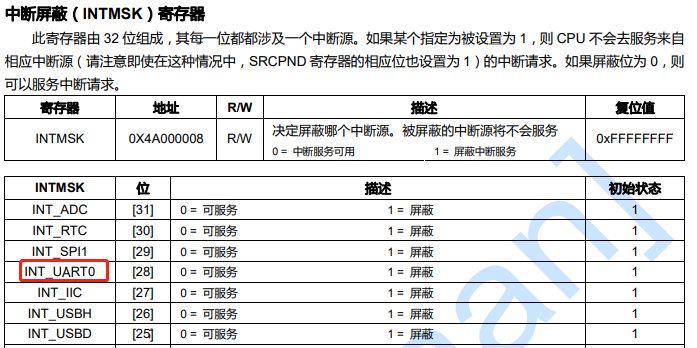
\includegraphics[width=0.7\textwidth]{uart4.png}
    \caption{INTMSK}
\end{figure}
\\
同时,由于我们还要定义是接收还是发送,也要打开INTSUBMSK,\\
\lstinline{INTSUBMSK &= ~(0x1);INTSUBMSK |= (0x1<<1);}
\begin{figure}[h]
    \centering
    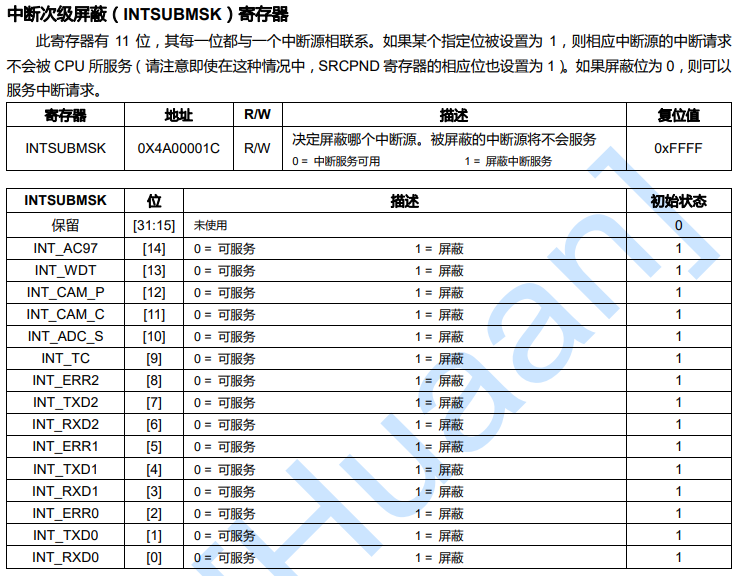
\includegraphics[width=0.7\textwidth]{uart5.png}
    \caption{INTSUBMSK}
\end{figure}

\subsection{结果}
当按下对应按键的时候,对方机子会亮对应的灯。
\begin{figure}[htbp]
    \centering
    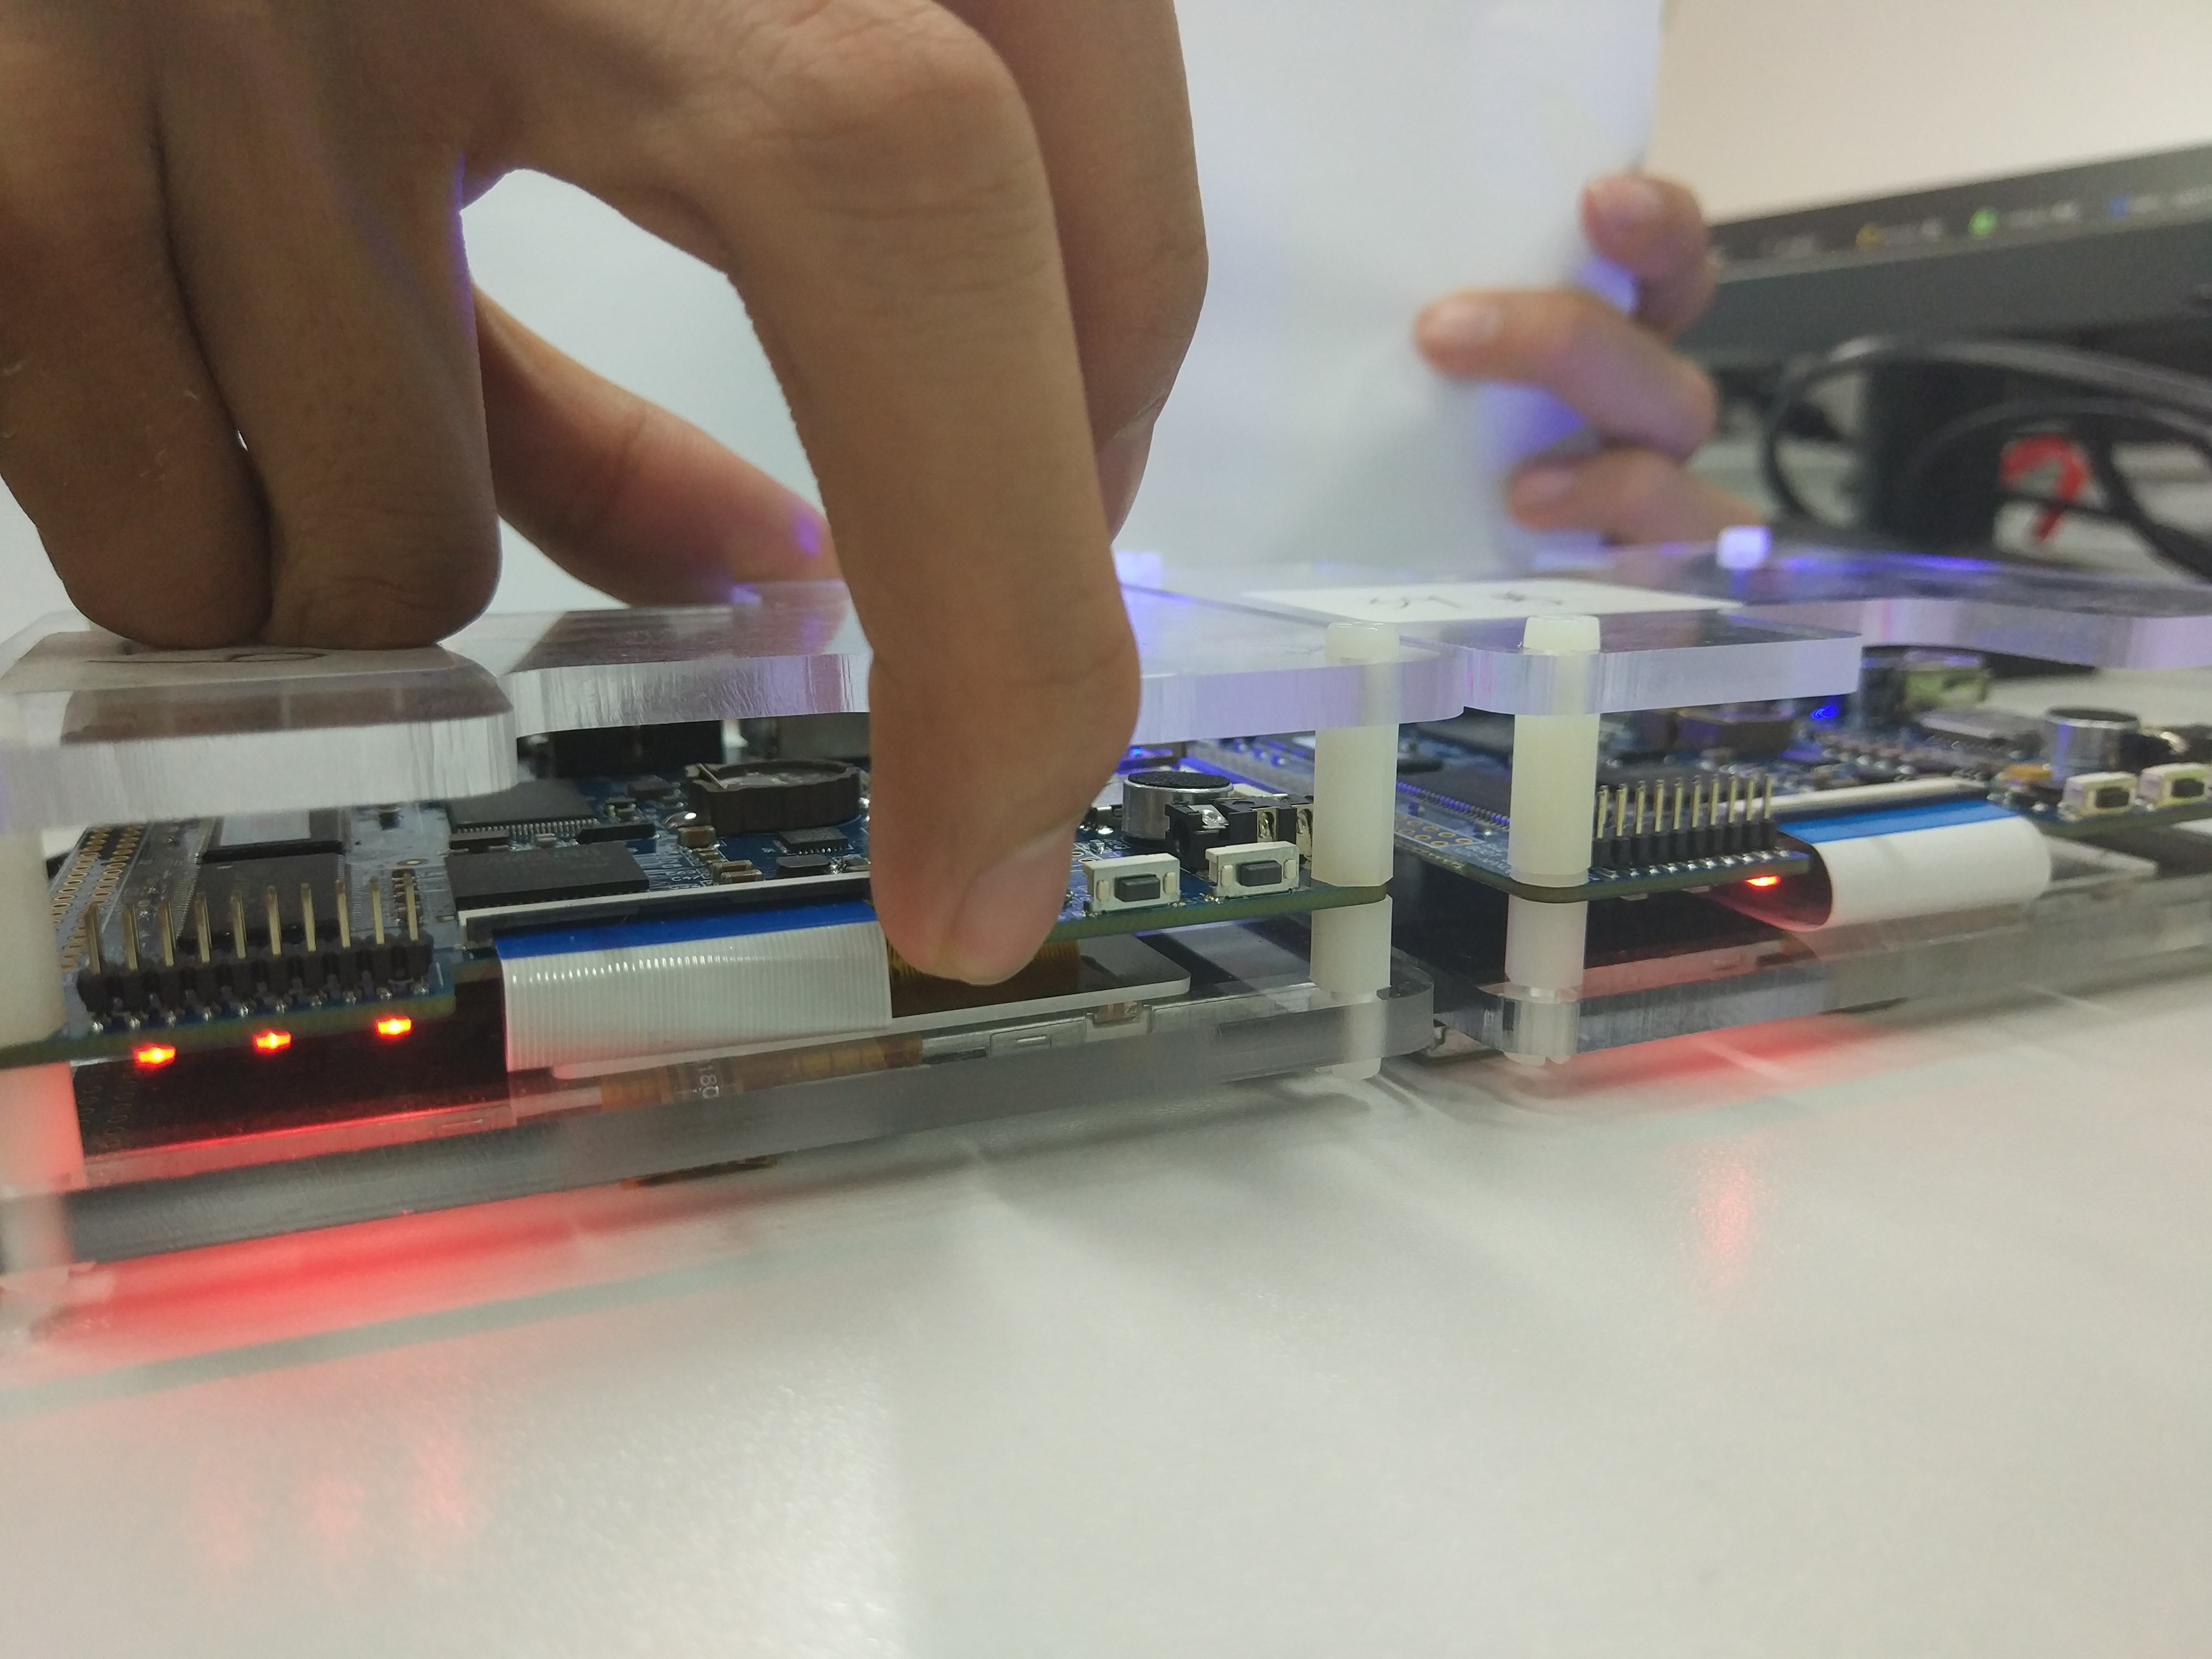
\includegraphics[width=0.5\textwidth]{result4-2}
    \caption{按下1号机子}
\end{figure}
\subsection{问题与总结}
仍然没能把两个中断写在同一个程序内,需要进一步改进。
